% Options for packages loaded elsewhere
% Options for packages loaded elsewhere
\PassOptionsToPackage{unicode}{hyperref}
\PassOptionsToPackage{hyphens}{url}
%
\documentclass[
  english,
  russian,
  12pt,
  a4paper,
  DIV=11,
  numbers=noendperiod]{scrreprt}
\usepackage{xcolor}
\usepackage{amsmath,amssymb}
\setcounter{secnumdepth}{5}
\usepackage{iftex}
\ifPDFTeX
  \usepackage[T1]{fontenc}
  \usepackage[utf8]{inputenc}
  \usepackage{textcomp} % provide euro and other symbols
\else % if luatex or xetex
  \usepackage{unicode-math} % this also loads fontspec
  \defaultfontfeatures{Scale=MatchLowercase}
  \defaultfontfeatures[\rmfamily]{Ligatures=TeX,Scale=1}
\fi
\usepackage{lmodern}
\ifPDFTeX\else
  % xetex/luatex font selection
\fi
% Use upquote if available, for straight quotes in verbatim environments
\IfFileExists{upquote.sty}{\usepackage{upquote}}{}
\IfFileExists{microtype.sty}{% use microtype if available
  \usepackage[]{microtype}
  \UseMicrotypeSet[protrusion]{basicmath} % disable protrusion for tt fonts
}{}
\usepackage{setspace}
% Make \paragraph and \subparagraph free-standing
\makeatletter
\ifx\paragraph\undefined\else
  \let\oldparagraph\paragraph
  \renewcommand{\paragraph}{
    \@ifstar
      \xxxParagraphStar
      \xxxParagraphNoStar
  }
  \newcommand{\xxxParagraphStar}[1]{\oldparagraph*{#1}\mbox{}}
  \newcommand{\xxxParagraphNoStar}[1]{\oldparagraph{#1}\mbox{}}
\fi
\ifx\subparagraph\undefined\else
  \let\oldsubparagraph\subparagraph
  \renewcommand{\subparagraph}{
    \@ifstar
      \xxxSubParagraphStar
      \xxxSubParagraphNoStar
  }
  \newcommand{\xxxSubParagraphStar}[1]{\oldsubparagraph*{#1}\mbox{}}
  \newcommand{\xxxSubParagraphNoStar}[1]{\oldsubparagraph{#1}\mbox{}}
\fi
\makeatother


\usepackage{longtable,booktabs,array}
\usepackage{calc} % for calculating minipage widths
% Correct order of tables after \paragraph or \subparagraph
\usepackage{etoolbox}
\makeatletter
\patchcmd\longtable{\par}{\if@noskipsec\mbox{}\fi\par}{}{}
\makeatother
% Allow footnotes in longtable head/foot
\IfFileExists{footnotehyper.sty}{\usepackage{footnotehyper}}{\usepackage{footnote}}
\makesavenoteenv{longtable}
\usepackage{graphicx}
\makeatletter
\newsavebox\pandoc@box
\newcommand*\pandocbounded[1]{% scales image to fit in text height/width
  \sbox\pandoc@box{#1}%
  \Gscale@div\@tempa{\textheight}{\dimexpr\ht\pandoc@box+\dp\pandoc@box\relax}%
  \Gscale@div\@tempb{\linewidth}{\wd\pandoc@box}%
  \ifdim\@tempb\p@<\@tempa\p@\let\@tempa\@tempb\fi% select the smaller of both
  \ifdim\@tempa\p@<\p@\scalebox{\@tempa}{\usebox\pandoc@box}%
  \else\usebox{\pandoc@box}%
  \fi%
}
% Set default figure placement to htbp
\def\fps@figure{htbp}
\makeatother



\ifLuaTeX
\usepackage[bidi=basic,provide=*]{babel}
\else
\usepackage[bidi=default,provide=*]{babel}
\fi
% get rid of language-specific shorthands (see #6817):
\let\LanguageShortHands\languageshorthands
\def\languageshorthands#1{}


\setlength{\emergencystretch}{3em} % prevent overfull lines

\providecommand{\tightlist}{%
  \setlength{\itemsep}{0pt}\setlength{\parskip}{0pt}}



 
\usepackage[backend=biber,langhook=extras,autolang=other*]{biblatex}
\addbibresource{bib/cite.bib}

\usepackage[]{csquotes}

\usepackage{indentfirst}
\usepackage{float}
\floatplacement{figure}{H}
\IfFileExists{plex-otf.sty}{
  %% Full TeXlive
  \IfPackageAtLeastTF{plex-otf.sty}{2024-12-06}{
    \usepackage[math,RM={Scale=0.94},SS={Scale=0.94},SScon={Scale=0.94},TT={Scale=MatchLowercase,FakeStretch=0.9},DefaultFeatures={Ligatures=Common}]{plex-otf}
  }{
    \usepackage[RM={Scale=0.94},SS={Scale=0.94},SScon={Scale=0.94},TT={Scale=MatchLowercase,FakeStretch=0.9},DefaultFeatures={Ligatures=Common}]{plex-otf}
  }
}{
  %% TinyTeX
  \usepackage{libertine}
}
\KOMAoption{captions}{tableheading}
\makeatletter
\@ifpackageloaded{caption}{}{\usepackage{caption}}
\AtBeginDocument{%
\ifdefined\contentsname
  \renewcommand*\contentsname{Содержание}
\else
  \newcommand\contentsname{Содержание}
\fi
\ifdefined\listfigurename
  \renewcommand*\listfigurename{Список иллюстраций}
\else
  \newcommand\listfigurename{Список иллюстраций}
\fi
\ifdefined\listtablename
  \renewcommand*\listtablename{Список таблиц}
\else
  \newcommand\listtablename{Список таблиц}
\fi
\ifdefined\figurename
  \renewcommand*\figurename{Рисунок}
\else
  \newcommand\figurename{Рисунок}
\fi
\ifdefined\tablename
  \renewcommand*\tablename{Таблица}
\else
  \newcommand\tablename{Таблица}
\fi
}
\@ifpackageloaded{float}{}{\usepackage{float}}
\floatstyle{ruled}
\@ifundefined{c@chapter}{\newfloat{codelisting}{h}{lop}}{\newfloat{codelisting}{h}{lop}[chapter]}
\floatname{codelisting}{Список}
\newcommand*\listoflistings{\listof{codelisting}{Листинги}}
\makeatother
\makeatletter
\makeatother
\makeatletter
\@ifpackageloaded{caption}{}{\usepackage{caption}}
\@ifpackageloaded{subcaption}{}{\usepackage{subcaption}}
\makeatother
\usepackage{bookmark}
\IfFileExists{xurl.sty}{\usepackage{xurl}}{} % add URL line breaks if available
\urlstyle{same}
\hypersetup{
  pdftitle={Шаблон отчёта по лабораторной работе},
  pdfauthor={Абрамян Жасмин},
  pdflang={ru-RU},
  hidelinks,
  pdfcreator={LaTeX via pandoc}}


\title{Шаблон отчёта по лабораторной работе}
\usepackage{etoolbox}
\makeatletter
\providecommand{\subtitle}[1]{% add subtitle to \maketitle
  \apptocmd{\@title}{\par {\large #1 \par}}{}{}
}
\makeatother
\subtitle{Работа с изображениями, размерами и плавающими объектами в
LaTeX}
\author{Абрамян Жасмин}
\date{}
\begin{document}
\maketitle

\renewcommand*\contentsname{Содержание}
{
\setcounter{tocdepth}{1}
\tableofcontents
}
\listoffigures
\listoftables

\setstretch{1.5}
\chapter{Цель
работы}\label{ux446ux435ux43bux44c-ux440ux430ux431ux43eux442ux44b}

Цель данной лабораторной работы --- изучить работу с изображениями в
LaTeX: научиться вставлять рисунки, управлять их размерами, положением и
подписями, использовать параметры \texttt{height}, \texttt{width},
\texttt{scale}, \texttt{angle} и понимать особенности размещения
плавающих объектов.

\chapter{Задание}\label{ux437ux430ux434ux430ux43dux438ux435}

Выполнить следующие упражнения:

\begin{enumerate}
\def\labelenumi{\arabic{enumi}.}
\tightlist
\item
  Включить собственное изображение, заменив стандартное, использованное
  в демонстрации.
\item
  Исследовать работу параметров \texttt{height}, \texttt{width},
  \texttt{angle} и \texttt{scale}.
\item
  Использовать ключ \texttt{width}, чтобы задать размер рисунка
  относительно \texttt{\textbackslash{}textwidth} и
  \texttt{\textbackslash{}linewidth}. Проверить, как это влияет при
  использовании опции \texttt{twocolumn}.
\item
  С помощью пакета \texttt{lipsum} создать длинный текст и
  протестировать различные спецификаторы размещения (\texttt{h},
  \texttt{t}, \texttt{b}, \texttt{p}, \texttt{{[}H{]}}) для объектов
  \texttt{figure}. Определить, как они влияют на положение изображений.
\item
  Добавить новые разделы, подразделы и нумерованные списки, а также
  проверить, сколько прогонов компиляции требуется, чтобы команды
  \texttt{\textbackslash{}label} и \texttt{\textbackslash{}ref} начали
  работать корректно.
\item
  Добавить несколько плавающих объектов и изучить, что произойдет, если
  \texttt{\textbackslash{}label} разместить \textbf{до} или
  \textbf{после} \texttt{\textbackslash{}caption}. Попробовать
  предсказать результат.
\item
  Проверить, что произойдет, если команда \texttt{\textbackslash{}label}
  для уравнения будет размещена \textbf{после}
  \texttt{\textbackslash{}end\{equation\}}.
\end{enumerate}

\chapter{Теоретическое
введение}\label{ux442ux435ux43eux440ux435ux442ux438ux447ux435ux441ux43aux43eux435-ux432ux432ux435ux434ux435ux43dux438ux435}

Работа с изображениями и плавающими объектами в LaTeX основана на
окружениях \texttt{figure}, \texttt{table} и командах
\texttt{\textbackslash{}includegraphics},
\texttt{\textbackslash{}caption}, \texttt{\textbackslash{}label}.

Основные параметры графики: - \texttt{width} --- ширина изображения
(например, \texttt{0.5\textbackslash{}textwidth}); - \texttt{height} ---
высота изображения; - \texttt{scale} --- масштаб изображения; -
\texttt{angle} --- угол поворота изображения.

\begin{figure}[h]
    \centering
    \includegraphics[width=0.5\textwidth, angle=10]
    \caption{Пример вставки изображения с изменением угла и ширины}
    \label
\end{figure}

Плавающие объекты управляются спецификаторами: - \texttt{h} (here) ---
«здесь»; - \texttt{t} (top) --- верх страницы; - \texttt{b} (bottom) ---
низ страницы; - \texttt{p} (page of floats) --- отдельная страница для
плавающих объектов; - \texttt{{[}H{]}} --- строго здесь (требуется пакет
\texttt{float}).

\begin{figure}

\centering{

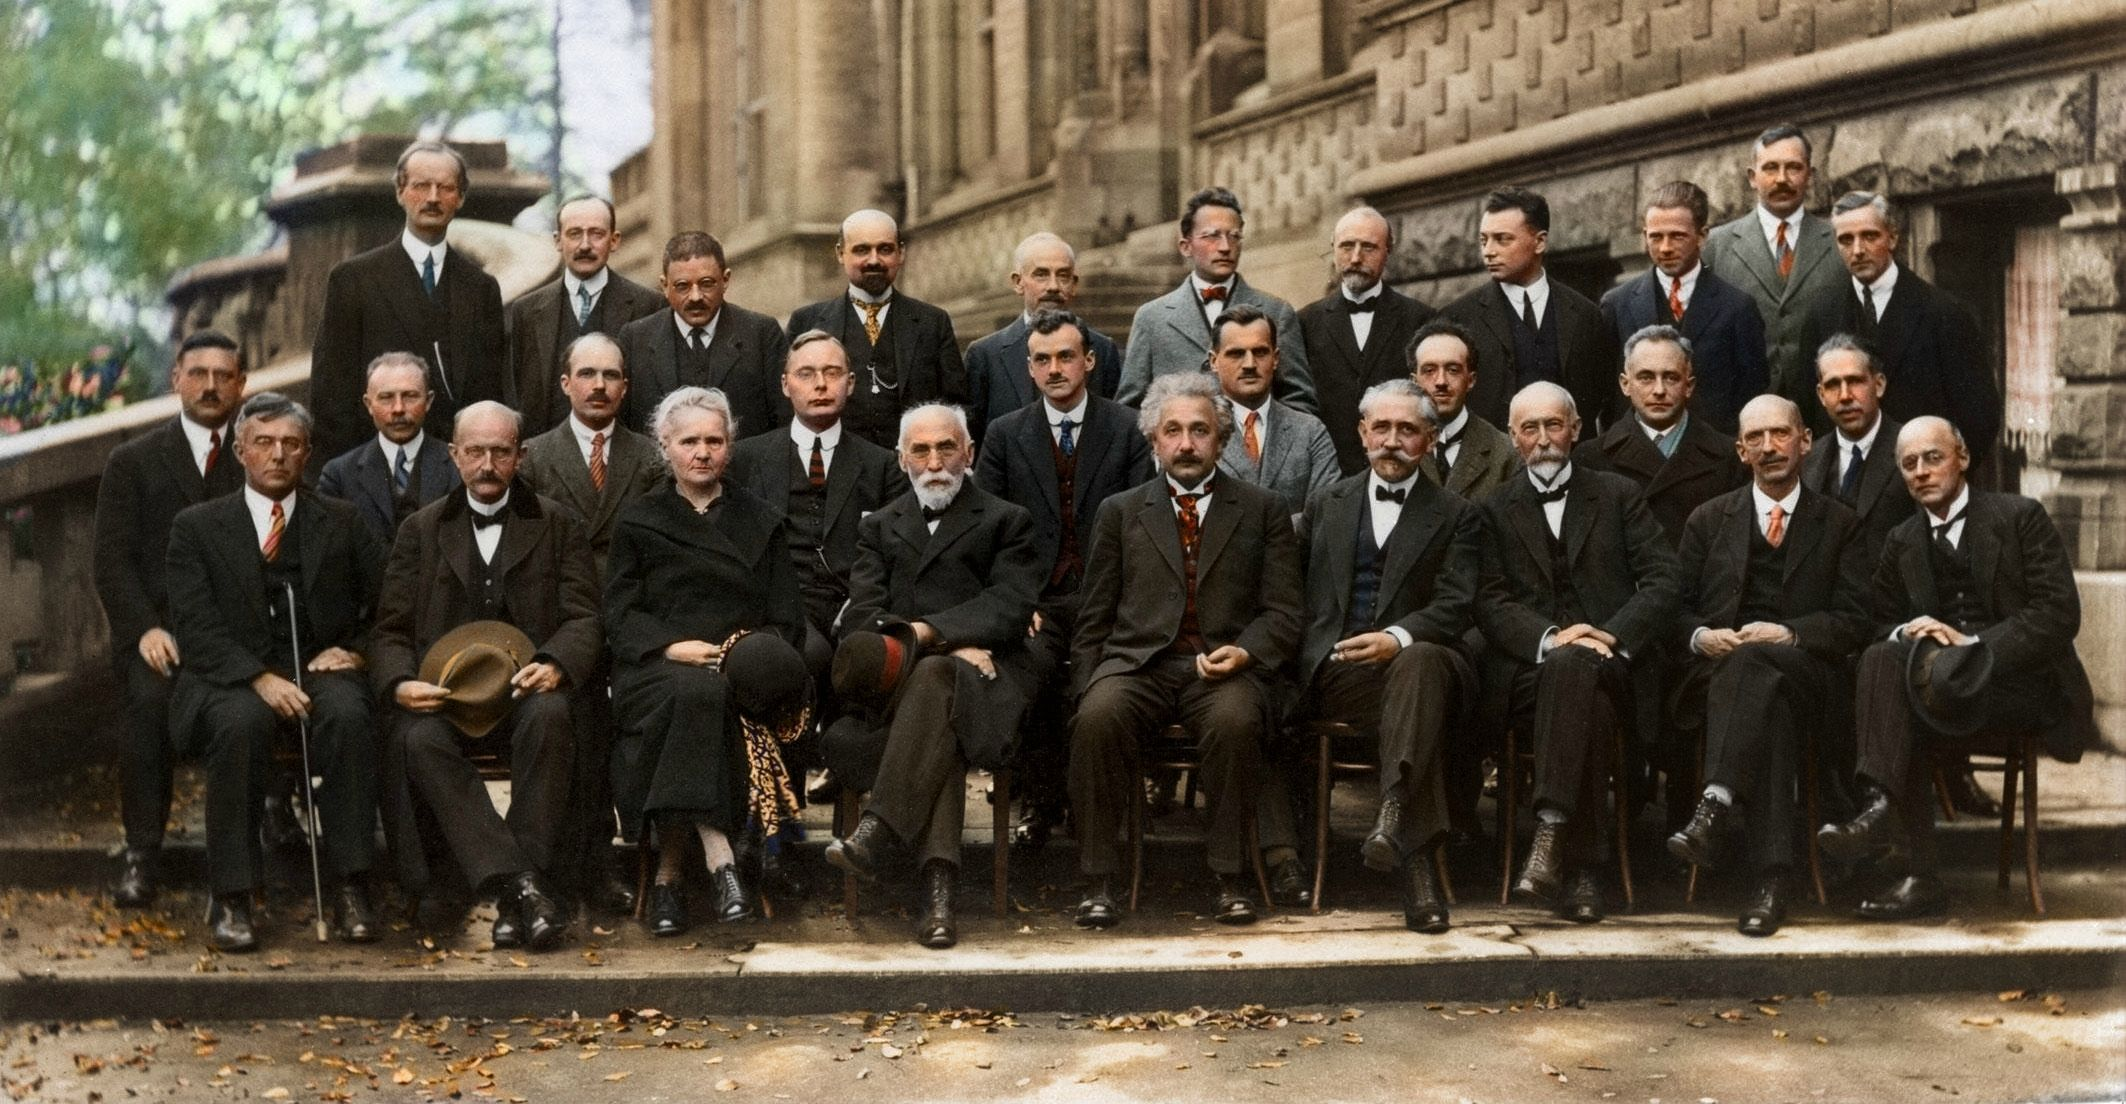
\includegraphics[width=0.6\linewidth,height=\textheight,keepaspectratio]{image/solvay.jpg}

}

\caption{\label{fig-001}}

\end{figure}%

\chapter{Выполнение лабораторной
работы}\label{ux432ux44bux43fux43eux43bux43dux435ux43dux438ux435-ux43bux430ux431ux43eux440ux430ux442ux43eux440ux43dux43eux439-ux440ux430ux431ux43eux442ux44b}

\begin{enumerate}
\def\labelenumi{\arabic{enumi}.}
\tightlist
\item
  Было добавлено три изображения в форматах \texttt{.jpg} с параметрами
  изменения ширины, угла и масштаба.
\item
  Проверено поведение рисунков при размещении в одно- и двухколоночных
  макетах.
\item
  Использованы команды \texttt{\textbackslash{}label} и
  \texttt{\textbackslash{}ref} для перекрёстных ссылок.
\item
  Проанализировано различие между размещением
  \texttt{\textbackslash{}label} до и после
  \texttt{\textbackslash{}caption}.
\item
  Проверено влияние позиции \texttt{{[}H{]}} при подключённом пакете
  \texttt{float}.
\end{enumerate}

\begin{figure}[H]
    \centering
    \includegraphics[width=0.7\linewidth]
    \caption{Положение [H] — здесь (требуется пакет float)}
    \label{fig:floatH}
\end{figure}

\chapter{Выводы}\label{ux432ux44bux432ux43eux434ux44b}

В результате выполнения работы: - освоены методы вставки и управления
изображениями в LaTeX; - изучены спецификаторы размещения
float-объектов; - проверена зависимость позиции от длины текста и макета
страницы; - отработаны навыки оформления отчётов с иллюстрациями,
ссылками и подписями.

\chapter*{Список
литературы}\label{ux441ux43fux438ux441ux43eux43a-ux43bux438ux442ux435ux440ux430ux442ux443ux440ux44b}
\addcontentsline{toc}{chapter}{Список литературы}

\printbibliography[heading=none]





\end{document}
